\documentclass[12pt]{article}
\usepackage[utf8]{inputenc}
\title{\vspace{-2.75cm}Technological Change and U.S. Foreign Aid\vspace{-0.5cm}}
\author{Nicholas Ray}
\date{\vspace{-0.30cm}December 7 2022\vspace{-1cm}}
\usepackage[margin=1in]{geometry}
\usepackage{mathtools,amssymb,amsthm}
\usepackage{setspace}
\doublespacing
\usepackage{footmisc}
\renewcommand{\footnotelayout}{\setstretch{1.75}}
\usepackage{footmisc}
\renewcommand{\footnotesize}{\normalsize}
\usepackage{caption}
\usepackage{tikz}
\usetikzlibrary{arrows,decorations.pathmorphing,backgrounds,fit,positioning,shapes.symbols,chains}
\usepackage{blindtext}
\usepackage{istgame}
\usepackage[backend=biber, style=authoryear, maxbibnames=99,uniquelist=false]{biblatex}
\renewbibmacro{in:}{}
\renewbibmacro*{volume+number+eid}{%
  \printfield{volume}
  \setunit*{\addnbthinspace}
  \printfield{number}
  \setunit{\addcomma\space}
  \printfield{eid}}
\DeclareFieldFormat[article]{number}{\mkbibparens{#1}}
\AtEveryBibitem{
  \clearfield{issn}
  \clearfield{month}
  \clearfield{urlyear}
  \clearlist{language}
  \clearfield{note}
  \clearfield{month}
  \clearfield{day}
  \ifentrytype{online}{}{
    \clearfield{url}
  }
}
\addbibresource{ForeignAidBib.bib}
\begin{document}
\maketitle
\begin{abstract}
    I argue that the U.S. is funding digital infrastructure in Africa to prevent the Chinese from building such infrastructure and closing market access to U.S. technology firms. Testing the implications that U.S. foreign aid spending is directly related to a measure for internet governance and inversely related to Chinese aid, I find mixed results in a sample of 44 African countries from 2010-2017. U.S. aid seems directly related to both internet governance and Chinese spending.
\end{abstract}

\textit{Keywords}: Foreign Aid, Internet Governance, Africa

\section*{Introduction}
The United States (U.S.) has been increasingly funding digital infrastructure in countries around the world.\footnote{All R code, data, and \LaTeX \;code can be found at  underlying my analysis can be found on GitHub at https://github.com/nnray.} Simultaneously, the People's Republic of China (China) has advanced its own digital infrastructure projects and financial assistance to become the ``lender of first resort'' for developing countries in the last decade \parencite[1]{dreher2022}. Available explanations do not sufficiently address this seeming great power competition along digital infrastructure. In this article I put forth an explanation specifying that the U.S. is funding digital infrastructure in Africa to prevent the Chinese from building such infrastructure and closing market access to U.S. technology firms.

I make two contributions in the exploration of this topic. Firstly, I add to the foreign aid literature by detailing a novel determinant of U.S. foreign aid and providing another clue on how Chinese money may have impacted Western donor behavior more generally. Secondly, I speak to literature on the liberal international order (LIO) and the concern that China may undermine tenets of the LIO. %expand on this a bit?

I proceed as follows. In the next section, I introduce puzzling observations of recent U.S. behavior followed by a review of current explanations. After considering these accounts, I introduce my argument its implications. Then, I describe my research design before presenting findings and a discussion of contributions.

\section*{What Needs Explaining}
%U.S. digital infrastructure spending, other aid related to ICT/internet
The U.S. has been increasingly funding digital infrastructure in countries around the world. In 2022, for example, the U.S. initiated the Partnership for Global Infrastructure and Investment (PGII) in collaboration with the other members of the Group of Seven (G7) that aims to spend \$600 billion on global infrastructure projects over the next five years (\cite{thewhitehouse2022}). Included in the PGII is a \$600 million contract to a U.S. telecommunications company to build submarine internet cables that connect Singapore to France via Egypt and the Horn of Africa. %other U.S. examples? IF programs? 

%Chinese digital infrastructure spending
This intention of the U.S. to build digital infrastructure closely resembles the behavior of China over the past two decades. Since engaging in their ``going out'' strategy of investing overseas to promote domestic economic growth, China has turned to funding massive infrastructure projects through its Belt and Road Initiative (BRI) and becoming the ``lender of first resort'' for developing countries \parencite[1]{dreher2022}. Two years after announcing the BRI, China launched the largely symbolic (\cite{tugendhat2021}) Digital Silk Road (DSR) that still encapsulates China's desire to build global digital infrastructure favorable to them (\cite{shen2022}). Some examples of relevant Chinese projects are shown in table 1 \nocite{agbebi2022}.

\subsubsection*{Table 1}
\begin{figure}[htbp]
    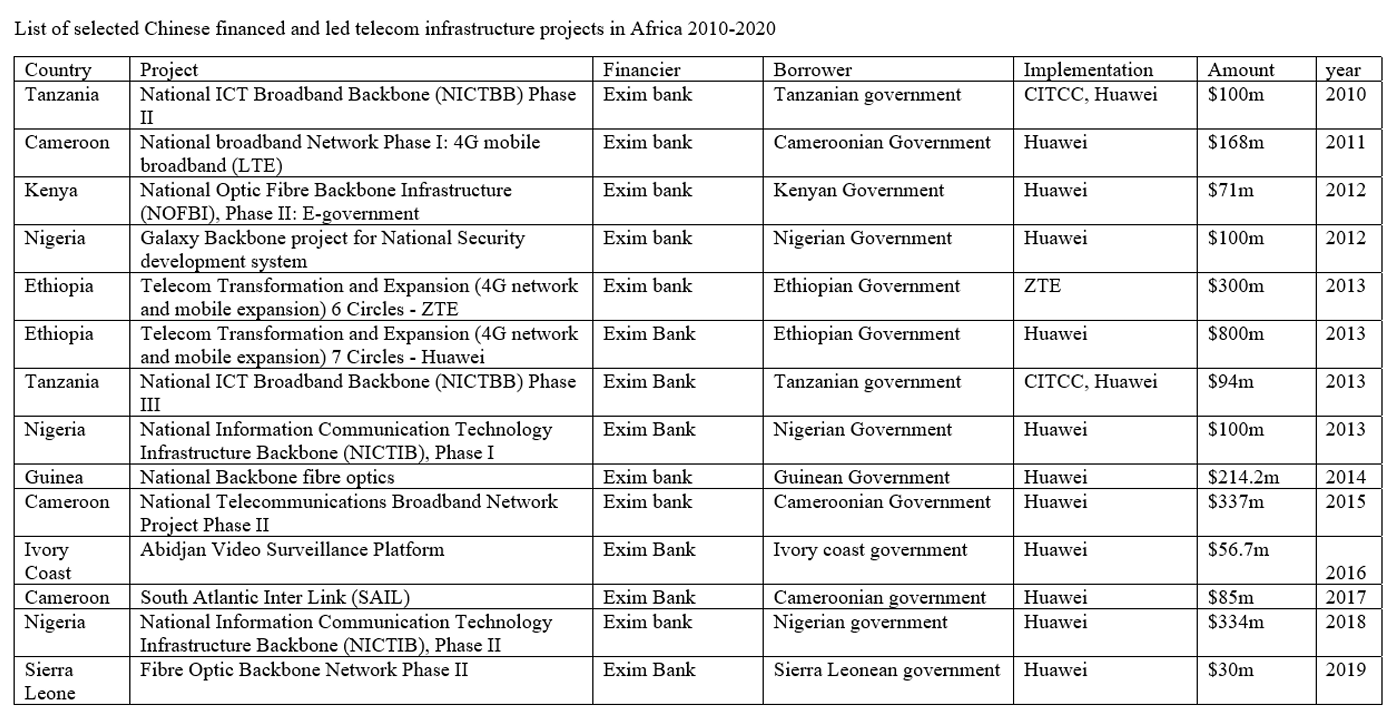
\includegraphics[scale=0.449]{Figures/ChineseAid.png}
    \captionof{table}{Agbebi 2022}
\end{figure}

%the competition between U.S. and Chinese technology, digital infrastructure spending
However, the U.S. and China do not seem to be cooperating in the effort to improve digital infrastructure worldwide. Just months before the PGII announcement, the U.S. pioneered a thinly veiled condemnation of China in the Declaration for the Future of the Internet in which more than 60 countries signed a pledge to engage in liberal internet governance (\cite{u.s.departmentofstate2022}). Further, policy analysts and scholars have a highlighted a U.S. concern over Chinese spending (\cite{hass2021}; \cite{triolo2020}; \cite{hillman2021}). Consequently, it appears that the U.S. and China are both separately spending on digital infrastructure projects while the U.S. actively opposes China's doing so.

\section*{Extant Explanations}
There are some tentative explanations offered by the global finance literature for this competitive spending behavior surrounding technology. For a comprehensive but not exhaustive overview of the literature on foreign aid determinants, see Fuchs, Dreher, and Nunnenkamp 2014 \nocite{fuchs2014} (Table 1, p. 173). Simplistically, the foreign aid literature has explained donor behavior as the result of either recipient need or self-interested motivations, with the self-interested reasons being categorizable as political or economic. Focusing on the determinants of U.S. foreign aid, I argue that the extant explanations do not fully capture either the technology focus of current U.S. aid behavior or the antagonistic nature of said behavior. 

There is evidence that the U.S. takes recipient need into account when allocating aid. Measured primarily as gross domestic product (GDP) per capita, Hoeffler and Outram (2011) \nocite{hoeffler2011} show that the U.S. spends more on poorer countries and that it matters little if there exists human rights abuses or non-democratic rule. Theoretically, U.S. spending on digital infrastructure could certainly contain some intention to meet recipient need and provide better technology, but it is not clear why the U.S. would be be in opposition to China's own digital infrastructure spending if that were the case. %mckinlay and buthe

The traditional account of U.S. aid behavior though focuses on self-interested motivations (e.g., \cite{mckinlay1977}). Economically, it has been theorized that the U.S. gives aid to countries that liberalize trade (\cite{alesina2000}) or export goods to the U.S. (\cite{younas2008}; \cite{fuchs2014}). It is also often stipulated that the U.S. is interested in economic growth (e.g., \cite{bearce2010b}). In this lighting, perhaps the U.S. is simply keen on stimulating economic growth in recipient countries since there is evidence that the internet is beneficial for developing economies (e.g., see \cite{wallsten2005}). However, economic motivations also do not explain why the U.S. should be opposed to Chinese spending. In fact, it would seem that the U.S. should theoretically be in favor of Chinese aid since there is evidence that Chinese aid procures economic growth in recipient countries (\cite{dreher2021}).

Politically, numerous authors highlight how counter-terrorism in the wake of the September 11$^{th}$ attacks resulted in an increase in U.S. aid after post-Cold War declines (e.g., \cite{fleck2010}; \cite{bearce2010b}). There have been mixed findings on how the democratic status of recipients and how voting records in the United Nations (UN) influences U.S. aid. Some scholars find a positive relationship between U.S. aid and recipient democracy (\cite{alesina2000}) or for the influence of similar UN voting patterns (\cite{alesina2000}; \cite{fuchs2014}), while others find substantially weaker evidence for both (\cite{hoeffler2011}). Meanwhile, there is no evidence that the U.S. factors in the human rights record of recipients (\cite{hoeffler2011}). It is possible that the U.S. is returning to a Cold War foreign aid mindset, where the aid they give is entirely concerned with strategically opposing their adversary (\cite{bearce2010b}). This would explain the antagonism with China, but not why there should be contention surrounding digital infrastructure and technology. %tingley, brech, fleck, dietrich

\section*{My Explanation}
I contend that an explanation of current U.S. foreign spending behavior must address both why it has a strong focus on technology and why this focus seems opposed to China. I argue that the U.S. is willing to spend aid on providing digital infrastructure because it allows them to build technology in U.S. fashion and thereby better protect U.S. technology market access to countries liable to Chinese technology influence. It is in the U.S.'s interest to attempt technological superiority over the Chinese, which is threatened by China's recent spreading of its technologies and companies to some recipient countries (see \cite{hass2021} for some suggestive anecdotal evidence).

If this is true, it should also be true that the U.S. is spending more in countries with more liberal internet governance since these are the countries that most allow for the use of U.S. technology. Further, these countries are likely not being invested in by China, whose aid is suspected on negatively affecting internet governance (e.g., \cite{triolo2020}; \cite{hillman2021}; \cite{u.s.departmentofstate2022}).

Internet governance was defined in the second phase of the World Summit on the Information Society (WSIS), a meeting led by the UN's International Telecommunication Union (ITU), which was held in Tunis, Tunisia in 2005. It is ``the development and application by governments, the private sector and civil society, in their respective roles, of shared principles, norms, rules, decision-making procedures, and programmes that shape the evolution and use of the Internet'' \nocite{worldsummitontheinformationsociety2005} (World Summit on the Information Society 2005, item 34). Essentially, internet governance refers to the way in which governments, firms, and citizens interact with the internet. The U.S. should be expected to allocate more aid to countries with higher measures of internet governance if they are truly bolstering U.S. firm access to technology markets.

\section*{Empirics}
Restating the implications of my argument, U.S. foreign aid should be directly related to recipient country internet governance since the U.S. is trying to build infrastructure that allows for an economically and politically liberal environment for U.S. technology to thrive. These same environments are most likely to exist in a country not financed by China, since China is sharing technology along with its money that could negatively affect recipient internet governance. Thus I will evaluate the following hypotheses:

\begin{align*}
    H_{1}&:\;\text{U.S. aid should be directly related to recipient internet governance}\\
    H_{2}&:\;\text{U.S. aid should be inversely related to Chinese aid}\\
\end{align*}
I test these hypotheses by regressing U.S. foreign aid on a measure of internet governance, Chinese aid and controls across 44 African countries between 2010 and 2017. The full set of countries includes: Algeria, Angola, Benin, Botswana, Burundi, Cabo Verde, Cameroon, Central African Republic, Chad, Comoros, Republic of the Congo, Cote d'Ivoire, Democratic Republic of the Congo, Djibouti, Egypt, Equatorial Guinea, Ethiopia, Gabon, Gambia, Ghana, Guinea, Guinea-Bissau, Kenya, Lesotho, Liberia, Madagascar, Malawi, Mali, Mauritania, Mauritius, Morocco, Mozambique, Namibia, Niger, Nigeria, Rwanda, Senegal, Sierra Leone, South Africa, Togo, Tunisia, Uganda, Zambia, and Zimbabwe. 

I chose to focus on Africa during this time period for three main reasons. Firstly, Africa has been a major area of focus for China's finance projects, with the Council on Foreign Relations claiming that ``China already provides more financing for information and communications technology than all multilateral agencies and leading democracies combined do across the continent'' (\cite{kurlantzicketal.2020}). Secondly, the data I use for Chinese spending ends in 2017. Thirdly, while 2010 is indeed an arbitrary starting point, it seems like a reasonable choice since both Chinese aid and the internet diminish greatly before this period.

\subsection*{Data and Variables}
%internet governance
In operationalizing my theory, I measure internet governance using the Digital Society Project (DSP) index. The DSP aims to identify ``how people use social media as a political tool and to explore how political institutions and social media use interact,'' providing data from expert surveys that cover a range of topics such as censorship, disinformation, and monitoring (\cite{mechkova2022}). The DSP employs methodology designed by the Varieties of Democracy project (V-Dem, \cite{coppedge2022}) to try and estimate differences in expert opinion and knowledge.

The DSP is one of two indices measuring a the concept of internet governance and data from the DSP is potentially superior for measuring the concept of internet liberalism in Africa compared to the primary alternative, Freedom on the Net (FOTN, \cite{freedomhouse2022}). FOTN frequently features missing data for the continent of Africa and does not take into account possible variations in expert opinion and knowledge like the DSP does.

%Chinese aid
The other main explanatory variable is Chinese foreign aid, stemming from the College of William \& Mary's AidData research lab (\cite{custer2021}). This is the one of the only datasets on Chinese aid and is certainly the largest and most specific. Aid is quantified as official financial and in-kind commitments and is collected using a methodology designed to track under-reported aid flows, such as those from China.

%U.S. aid
U.S. foreign aid is the dependent variable, measured as fiscal-year disbursements (\cite{u.s.agencyforinternationaldevelopment2022}). This data was more up-to-date than alternatives.

%controls
For controls, I include gross domestic product GDP per capita, an indicator for internet development, and a measure for political freedom as controls. Each of these phenomena are possible confounders, being theoretically related to at least one of the types of aid and internet governance. 

GDP per capita is supplied by the United Nations (\cite{unitednationsstatisticsdivision2019}) while the indicator for internet development is provided by the ITU (\cite{internationaltelecommunicationunion2022}). This indicator is a proxy for how developed the internet is in a country and represents the percentage of the population using the internet. Lastly, the chosen measure for political freedom comes from Polity (\cite{marshall2018}).

Using a GDP deflator (\cite{organizationforeconomicco-operationanddevelopment2022}), the values for U.S. aid, Chinese aid, and GDP per capita are all in constant 2015 USD.

%Missing data
Of the 10 African countries I am missing data for, the DSP is missing values for Somalia, Eritrea, Sudan, and South Sudan, which might make sense given that Somalia and South Sudan were both at civil war during the observation period while Sudan and Eritrea have experienced instability after previous wars. Similarly, Libya was missing data from the ITU following the Western invasion of Libya in 2011. However, it is unclear why Sao Tome and Principe and Seychelles are missing Polity data, why Burkina Faso and Eswatani are missing Chinese aid data, or why Tanzania is missing GDP data.

%add discussion of larger descriptive stats table
Descriptive statistics can be seen in table 2 and 3 below. It should be noted that the variable logged Chinese aid is mostly zeroes, as can be seen again in figure 4. I performed Grubbs' tests for outliers and indeed, the highest values for logged Chiense aid are outliers from the modal zero. All other variables, though, support ample variation and are stationary or trendstationary by themselves. 

\subsubsection*{Table 2}
\begin{figure}[htbp]
    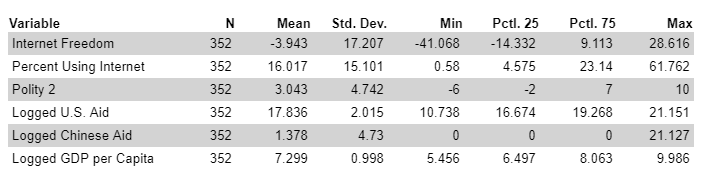
\includegraphics[scale=0.8]{Figures/628table2.png}
\end{figure}
\pagebreak

\subsubsection*{Table 3}
\begin{figure}[htbp]
    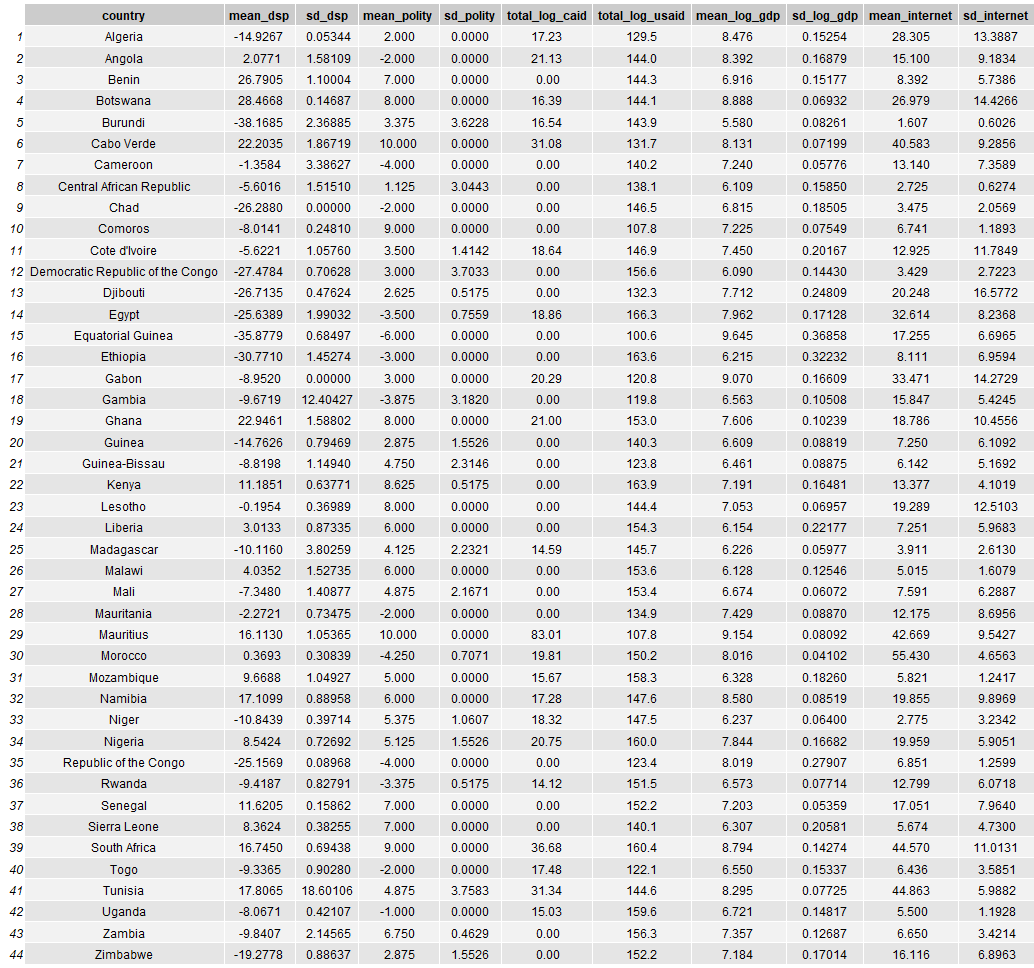
\includegraphics[scale=0.45]{Figures/summary.png}
\end{figure}

\pagebreak
A correlation matrix of the variables included in my regressions is given in Figure 2. As can be seen, there are a couple relatively strong relationships between the variables. The variable for regime type, Polity, has a correlation of 0.62 with the internet governance variable while logged GDP per capita has a correlation of 0.65 with the variable representing the percent of the population using the internet. While possible, I do not think that these correlations are high enough to warrant concerns over multicollinearity or the lack of linear independency in the data. Interestingly, logged U.S. Aid appears somewhat negatively correlated with logged GDP per capita and variable for the percent using the internet is somewhat positively correlated to that for internet governance. However, all of these correlations are relatively small and should not induce concerns for multicollinearity, although I did not conduct a formal test for multicollinearity.

\pagebreak
\subsubsection*{Figure 2}
\begin{figure}[htbp]
    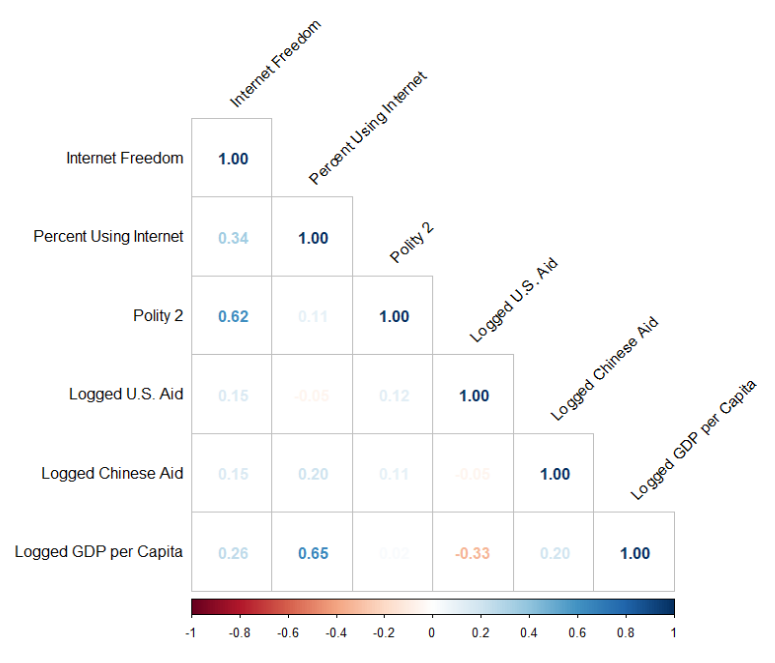
\includegraphics[scale=0.7]{Figures/628plot3.png}
\end{figure}

\subsection*{Estimation}
I chose to use ordinary least squares (OLS) for my estimator while employing two-way fixed effects at the country and year level. In choosing fixed effects, I used non-nested model comparison tests that suggested fixed effects to be superior to both no effects and random effects. After testing for heteroskedasticity, I included country-clustered standard errors. %look at the as.factor(years) as evidence of relationship getting stronger over time?

\pagebreak
\section*{Results}
Table 2 displays regression results from a model with and without an interaction between internet governance and logged Chinese foreign aid.
\begin{table}[!htbp] \centering 
  \caption{Logged U.S. Aid and Covariates with Two-way Fixed Effects and Clustered SE's on Country} 
  \label{} 
\begin{tabular}{@{\extracolsep{5pt}}lcc} 
\\[-1.8ex]\hline 
\hline \\[-1.8ex] 
 & \multicolumn{2}{c}{Logged U.S. Aid} \\ 
\cline{2-3} 
 & Model 1 & Model 2 \\ 
\hline \\[-1.8ex] 
 Internet Governance & 0.021$^{***}$ & 0.021$^{***}$ \\ 
  & (0.008) & (0.008) \\ 
  & & \\ 
 Logged Chinese Aid & 0.006$^{*}$ & 0.006$^{*}$ \\ 
  & (0.003) & (0.003) \\ 
  & & \\ 
 Logged GDP per Capita & 0.045 & 0.045 \\ 
  & (0.471) & (0.472) \\ 
  & & \\ 
 Percent Using Internet & $-$0.013 & $-$0.013 \\ 
  & (0.009) & (0.009) \\ 
  & & \\ 
 Polity & 0.004 & 0.004 \\ 
  & (0.031) & (0.031) \\ 
  & & \\ 
 Internet Governance * Logged Chinese Aid &  & 0.00000 \\ 
  &  & (0.0002) \\ 
  & & \\ 
\hline \\[-1.8ex] 
Observations & 352 & 352 \\ 
R$^{2}$ & 0.038 & 0.038 \\ 
Adjusted R$^{2}$ & $-$0.140 & $-$0.144 \\ 
F Statistic & 2.370$^{**}$ (df = 5; 296) & 1.968$^{*}$ (df = 6; 295) \\ 
\hline 
\hline \\[-1.8ex] 
\textit{Note:}  & \multicolumn{2}{r}{$^{*}$p$<$0.1; $^{**}$p$<$0.05; $^{***}$p$<$0.01} \\ 
\end{tabular} 
\end{table}
\pagebreak

The only covariates that appear statistically significant are internet governance and Chinese spending. Both internet governance and logged Chinese aid seem to increase logged U.S. aid on average when accounting for the other covariates. To gauge the substantive size of the coefficients, I plot the marginal effect of internet governance on logged U.S. aid in Figure 3 and the marginal effect of logged Chinese aid on logged U.S. aid in Figure 4, both from model 1 (seen in Table 2).

According to Table 2 and Figures 3 and 4, there is support for $H_1$. $H_2$ is contradicted by the evidence, meanwhile. However, I would be cautious about inferences from the results pertaining to logged Chinese aid as most of the values are zero, as can be seen in Figure 4. It is thus likely that the downward sloping line is overestimated due to all the zeros.

I also tested for an interaction between internet governance and logged Chinese aid, which was not part of my theory. The interaction term is not significant according to standard levels (p=0.05).

\pagebreak
Figure 3 shows the marginal effect of internet governance on logged U.S. foreign aid. The coefficient on the internet governance variable is 0.0206, implying that a one unit increase in a recipient's internet governance level is associated with an increase in U.S. aid by 2.08 percent on average, accounting for other covariates. This appears to be a substantively large effect.

\subsection*{Figure 3}
\begin{figure}[htbp]
    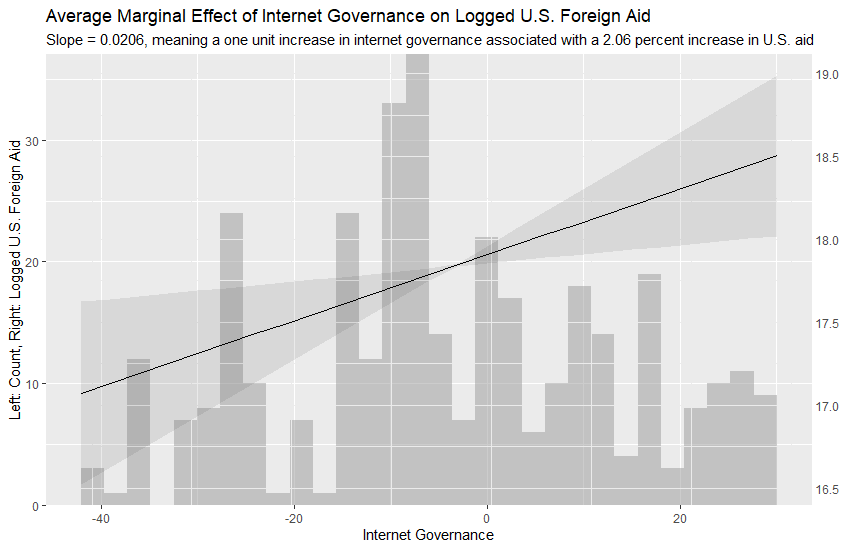
\includegraphics[scale=0.7]{Figures/628plot1.png}
\end{figure}

\pagebreak
Figure 4 graphs the marginal effect of logged Chinese foreign aid on logged U.S. foreign aid. The coefficient on the variable for logged Chinese foreign aid is 0.0058, implying that a one percent increase in Chinese aid is associated with a 0.0058 percent increase in U.S. aid on average, accounting for other covariates. This does not appear to be a substantively large effect.

\subsection*{Figure 4}
\begin{figure}[htbp]
    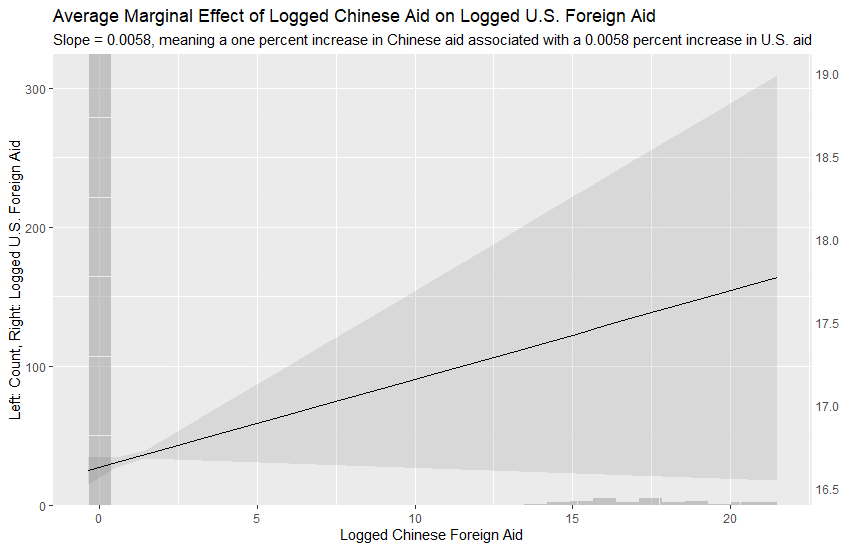
\includegraphics[scale=0.7]{Figures/628plot2.png}
\end{figure}
\pagebreak 

\section*{Discussion}
The support of $H_1$ but not $H_2$ indicate mixed results for my theory. However, it seems that robustness checks with mulitple other measures would be required to make more inferences about U.S. behavior, including for regime type and especially Chinese aid. The variable for Chinese aid contains mostly zeros with a few, large values that are qualified as outliers.

To the extent that my theory is supported, I contribute to the foreign aid literature by detailing a potentially new determinant for U.S. behavior. The internet and technology as a foreign policy and geopolitical issue will only continue to rise, and it's important that scholarly theories keep pace with contemporary observation. Secondly, some international relations literature has expressed concerns that China will undermine common tenets of the LIO, such as economic or political liberalism (e.g., \cite{weiss2021a}). While I do not study China's behavior here, my analysis indicate somewhat that the U.S. behaves as if China is indeed damaging political and economic liberalism, especially as it relates to the liberal use of the internet.

\section*{Conclusion}
In this article I argue that the U.S. is funding digital infrastructure in Africa to prevent the Chinese from building such infrastructure and closing market access to U.S. technology firms. I test the implications that U.S. foreign aid spending should be directly related to a measure for internet governance, or the rules and norms surrounding the internet, and inversely related to Chinese aid spending.

Analyzing 44 African countries from 2010-2017, I find mixed results for the theory, as U.S. aid indeed seems directly related to internet governance but also directly related to Chinese spending.

In future work, other measures for Chinese spending and influence would be critical to analyzing their digital infrastructure activities in Africa that go poorly reflected in aid data. The deriving of other implications and more falsification attempts are also necessary to test this explanation for recent U.S. spending behavior. 

\nocite{mechkova2022a}
\nocite{pemstein2022}
\nocite{coppedge2022}
\nocite{coppedge2022a}
\nocite{coppedge2022b}
\nocite{coppedge2022c}
\nocite{coppedge2022d}
\nocite{curini2020}
\pagebreak
\printbibliography
\end{document}